\section{Quantum Capacity of Quantum Channels}

\subsection{Coherent Information and Quantum Capacity}

We now concern ourselves with the transmission of quantum states. Recall that both classical and private communication models concerned themselves with reliable transmission of classical bits. This was typically modelled with orthogonal basis states. However, transmission of arbitrary quantum states involve dealing with more complex phenomenon such as entanglement.

Suppose Alice prepares a pure state $\phi_{AA'}$ and inputs the system $A'$ to a quantum channel $\mathcal{N}_{A' \rightarrow B}$. This transmission gives us the bipartite state $\rho_{AB} = \mathcal{N}_{A' \rightarrow B} (\phi_{AA'})$. An intuitive way of measuring the information throughput is to measure how uncertain the receiver is of the input given the received quantum state. This aligns with the definiton of conditional entropy. Since we are concerned with reducing the conditional entropy, we can define an analogous measure that can be maximized instead.

\begin{definition}[Coherent Information of a Quantum State]
The coherent information of a bipartite state $\rho_{AB} \in \mathcal{D}(\mathcal{H}_A \otimes \mathcal{H}_B)$ is defined as:
$$I(A \rangle B)_{\rho} = S(B)_{\rho} - S(AB)_{\rho}$$
\end{definition}

\begin{definition}[Quantum Capacity of a Quantum Channel]
The quantum information $Q(\mathcal{N})$ of a quantum channel $\mathcal{N}$ is defined as:
\begin{align*}
Q(\mathcal{N}) &= \max_{\phi_{AA'}} \left[ I(A \rangle B)_{\rho} \right] \\
&= \max_{\phi_{AA'}} \left[ S(B)_\rho - S(AB)_\rho \right]
\end{align*}
\end{definition}

\noindent An equivalent way of writing the quantum capacity is as follows, where $\ket{\psi}_{ABE} = U_{A' \rightarrow BE}^{\mathcal{N}} \ket{\phi}_{AA'}$.
$$Q(\mathcal{N}) = \max_{\phi_{AA'}} \left[ S(B)_\psi - S(E)_\psi \right]$$

\begin{figure}[H]
    \centering
    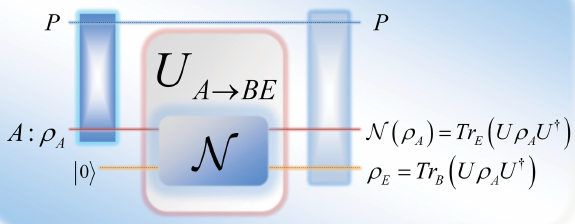
\includegraphics[width=0.6\textwidth]{figures/quantum_communication_quantum_channel.png}
    \caption{Quantum communication through a quantum channel \cite{Gyongyosi_2018}. The channel is represented as the unitary transformation. $P$ refers to the reference system or the purification state. The outputs received by Bob (first) and the environment (second) can be computed using the partial trace operator.}
\end{figure}

We shall see that this definition of quantum capacity satisifies non-negativity, but violates the additivity relation similar to private capacity. We would then examine a special class of quantum channels that satisfies the additive relation for both private and quantum capacity. Moreover, their private and quantum capacities happen to be always equal.

\subsection{Properties of Quantum Capacity}

\begin{theorem}[Non-negativity]
The quantum capacity $Q(\mathcal{N})$ of a quantum channel $\mathcal{N}$ is non-negative.
$$Q(\mathcal{N}) \geq 0$$
\end{theorem}

\begin{proof}
Similar to the non-negativity proofs earlier, we would construct a state that achieves zero coherent information. Since the quantum capacity is the maximum over all such states, it is guaranteed to be non-negative.

Consider the input state $\phi_{AA'}$ to be a product state of the form $\psi_A \otimes \Phi_{A'}$, where the state $A$ is pure. We can evaluate its coherent information as follows.

\begin{align*}
I(A \rangle B)_{\psi \otimes \mathcal{N}(\Phi)} &= S(B)_{\mathcal{N}(\Phi)} - S(AB)_{\psi \otimes \mathcal{N}(\Phi)} \\
&= S(B)_{\mathcal{N}(\Phi)} - S(A)_{\psi} - S(B)_{\mathcal{N}(\Phi)} \\
&= - S(A)_{\psi} \\
&= 0
\end{align*}

The first equality follows from the definition of coherent information. The second makes use of the fact that $AB$ is a product state. The third cancels out common terms, while the fourth makes use of the fact that $A$ is a pure state.
\end{proof}

\begin{theorem}[Non-additivity]
Let $\mathcal{N}_1$ and $\mathcal{N}_2$ represent two quantum channels. The quantum capacity of the combined quantum channel $\mathcal{N}_1 \otimes \mathcal{N}_2$ is not equal to the sum of the individual quantum capacities of $\mathcal{N}_1$ and $\mathcal{N}_2$.
$$Q(\mathcal{N}_1 \otimes \mathcal{N}_2) \neq Q(\mathcal{N}_1) + Q(\mathcal{N}_2)$$
\end{theorem}

\begin{proof}
Consider a private Horodecki channel $\mathcal{N}_H$ and a symmetric channel of unbounded dimension $\mathcal{A}$. These channels are known to have the following properties \cite{Horodecki_1996} \cite{Horodecki_1997} \cite{Smith_2008_Symmetric}.
$$P(\mathcal{N}_H) > 0, Q(\mathcal{N}_H) = 0, Q(\mathcal{A}) = 0$$

Further, we will utilize the following relation between the private capacity and the assisted capacity \cite{Smith_2008}.
$$\frac{1}{2} P(N_H) \leq Q_\mathcal{A}(N_H)$$

Since $P(\mathcal{N}_H) > 0$, it follows that the assisted capacity $Q_\mathcal{A}(\mathcal{N}_H) > 0$. Further, since $\mathcal{A}$ is a symmetric channel of unbounded dimension, the quantum capacity of the joint channel can be related with the assisted capacity as follows \cite{Smith_2008_Symmetric}.
$$Q(\mathcal{N}_H \times \mathcal{A}) = Q_\mathcal{A}(\mathcal{N}_H) > 0$$

Finally, note that $Q(\mathcal{N}_H) + Q(\mathcal{A}) = 0$. We can thus conclude the following relation establishing non-additivity.
$$Q(\mathcal{N}_H \times \mathcal{A}) \neq Q(\mathcal{N}_H) + Q(\mathcal{A})$$
\end{proof}

\begin{theorem}[Relation with other capacities]
The single use capacities of a quantum channel $\mathcal{N}$ are related to each other as:
$$Q(\mathcal{N}) \leq P(\mathcal{N}) \leq C(\mathcal{N})$$
\end{theorem}

\begin{proof}
The reason why $P(\mathcal{N}) \leq C(\mathcal{N})$ holds is easy to see. In both classical and private communication models, our objective is to transmit classical information. Private communication is a specific case of the lesser constrained classical communication through quantum channels. Thus, the classical capacity cannot be lesser than the private capacity.

For proving the other half of the inequality, i.e. $Q(\mathcal{N}) \leq P(\mathcal{N})$, we will consider a pure state that maximizes the quantum capacity. Let $\sigma_{XA'}$ denote the augmented classical-quantum state that correlates with index $x$.

$$\sigma_{XA'} = \sum_{x} p_X(x) \ket{x}\bra{x} \otimes \ket{\phi_x}\bra{\phi_x}_{A'}$$

\begin{align*}
Q(\mathcal{N}) &= \max_{\rho} \left[ S(B)_{\rho} - S(E)_{\rho} \right] \\
&= S(B)_{\sigma} - S(E)_{\sigma} \\
&= S(B)_{\sigma} - S(B|X)_{\sigma} - S(E)_{\sigma} + S(B|X)_{\sigma} \\
&= I(X;B)_{\sigma} - S(E)_{\sigma} + S(E|X)_{\sigma} \\
&= I(X;B)_{\sigma} - I(X;E)_{\sigma} \\
&\leq \max_{\rho} \left[ I(X;B)_{\rho} - I(X;E)_{\rho} \right] \\
&= P(\mathcal{N})
\end{align*}
\end{proof}

The first equality is by definition of quantum capacity. The second equality is by construction of the quantum state. The fourth equality is by the definition of mutual information and by the fact that $\sigma$ on systems $B$ and $E$ is pure when conditioned on $X$. The fifth equality is by the definition of mutual information. The last equality is by the definition of private capacity.

\subsection{Degradable Quantum Channels}

A channel $\mathcal{N}: \mathcal{H}_A \rightarrow \mathcal{H}_B$ can be defined by an isometric embedding $U: \mathcal{H}_A \rightarrow \mathcal{H}_B \otimes \mathcal{H}_E$, followed by a partial trace over the environment system $E$: $\mathcal{N}(\rho) = \mathrm{Tr}_E U(\rho)$. The complementary channel $\mathcal{N}^c: \mathcal{H}_A \rightarrow \mathcal{H}_E$ is defined by: $\mathcal{N}^c(\rho) = \mathrm{Tr}_B U(\rho)$. We regard a quantum channel as degradable if the transmission from the sender end to the environment is noisier than the transmission to the receiver. This is modeled as a result of an additional application of a ``degrading'' channel.

\begin{figure}[H]
    \centering
    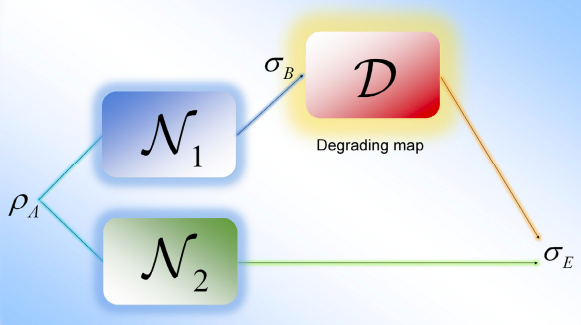
\includegraphics[width=0.6\textwidth]{figures/degradable_quantum_channel.png}
    \caption{The concept of a degradable quantum channel \cite{Gyongyosi2012PropertiesOT}. The environment state can be simulated by the application of the degrading channel on the quantum state received by Bob.}
\end{figure}

\begin{definition}[Degradable Quantum Channel]
A channel $\mathcal{N}: \mathcal{H}_A \rightarrow \mathcal{H}_B$ is called degradable when it may be degraded to its complementary channel $\mathcal{N}^c: \mathcal{H}_A \rightarrow \mathcal{H}_E$, i.e. when there exists a CPTP map $T: \mathcal{H}_B \rightarrow \mathcal{H}_E$ such that
$$\mathcal{N}^c = T \circ \mathcal{N}$$
\end{definition}

\begin{theorem}[Additivity of Quantum Capacity]
Let $\mathcal{N}$ and $\mathcal{M}$ represent two degradable quantum channels. The quantum capacity of the combined quantum channel $\mathcal{N} \otimes \mathcal{M}$ is equal to the sum of the individual quantum capacities of $\mathcal{N}$ and $\mathcal{M}$.
$$Q(\mathcal{N} \otimes \mathcal{M}) = Q(\mathcal{N}) + Q(\mathcal{M})$$
\end{theorem}

\begin{proof}
The reason why $Q(\mathcal{N} \otimes \mathcal{M}) \geq Q(\mathcal{N}) + Q(\mathcal{M})$ holds is easy to see. We can think of a separable input state $\rho_{AB} = \rho_A \otimes \rho_B$ that is maximized indepedently for the two channels. Since the entropy is additive for such states, the joint capacity cannot be lower than the sum of invididual capacities. 

For the reverse direction, consider a pure state $\phi_{AA_1'A_2'}$ as the input to the two channels. Let the following denote the result of the channels, where $\rho_{AB_{1}E_{1}B_{2}E_{2}}$ is a state that maximizes $Q(\mathcal{N} \otimes \mathcal{M})$.
\begin{align*}
\sigma_{AB_{1}E_{1}A_{2}} &= U^{N} \phi (U^{N})^{\dagger} \\
\theta_{AA_{1}B_{1}E_{2}} &= U^{M} \phi (U^{M})^{\dagger} \\
\rho_{AB_{1}E_{1}B_{2}E_{2}} &= (U^{N} \otimes U^{M}) \phi ((U^{N})^{\dagger} \otimes (U^{M})^{\dagger})
\end{align*}

We can write the quantum capacity of the joint channel as follows to show the reverse direction.
\begin{align*}
Q(\mathcal{N} \otimes \mathcal{M}) &= I(A;B_1B_2)_{\rho} \\
&= S(B_1B_2)_{\rho} - S(E_1E_2)_{\rho} \\
&= S(B_1)_{\rho} - S(E_1)_{\rho} + S(B_2)_{\rho} - S(E_2)_{\rho} - [I(B_1;B_2)_{\rho} - I(E_1;E_2)_{\rho}] \\
&\leq S(B_1)_{\rho} - S(E_1)_{\rho} + S(B_2)_{\rho} - S(E_2)_{\rho} \\
&= S(B_1)_{\sigma} - S(AA_2'B_1)_{\sigma} + S(B_2)_{\sigma} - S(AA_1'B_2)_{\sigma} \\
&= I(AA_2';B_1)_{\sigma} + I(AA_1';B_2)_{\sigma} \\
&\leq Q(\mathcal{N}) + Q(\mathcal{M})
\end{align*}

The fourth inequality holds because there is a degrading channel from both $B_1$ to $E_1$ and $B_2$ to $E_2$. This gives us $I(B_1; B_2)_\rho \geq I(E_1; E_2)_\rho$. The fifth inequality holds because the state $\sigma$ on systems $AA_2'B_1E_1$ is pure and the state $\theta$ on systems $AA_1'B_2E_2$ is pure.

Combining the two inequalities establishes the additivity of quantum capacity of degradable channels.
\end{proof}

\begin{theorem}[Additivity of Private Capacity]
Let $\mathcal{N}$ and $\mathcal{M}$ represent two degradable quantum channels. The private capacity of the combined quantum channel $\mathcal{N} \otimes \mathcal{M}$ is equal to the sum of the individual private capacities of $\mathcal{N}$ and $\mathcal{M}$.
$$P(\mathcal{N} \otimes \mathcal{M}) = P(\mathcal{N}) + P(\mathcal{M})$$
\end{theorem}

\begin{proof}
To prove $P(\mathcal{N} \otimes \mathcal{M}) \geq P(\mathcal{N}) + P(\mathcal{M})$, consider the states $\rho$ and $\sigma$ maximizing the private capacity of channels $\mathcal{N}$ and $\mathcal{M}$ respectively. Let $\theta = \rho \otimes \sigma$ be the tensor product of the two states. Then using the additivity of mutual information on tensor product states, we can write the following.
\begin{align*}
P(\mathcal{N}) + P(\mathcal{M}) &= I(X_1;B_1)_{\rho} - I(X_1;E_1)_{\rho} + I(X_2;B_2)_{\sigma} - I(X_2;E_2)_{\sigma} \\
&= I(X_1X_2;B_1B_2)_{\theta} - I(X_1X_2;E_1E_2)_{\theta} \\
&\leq \max_{\alpha} \left[ I(X_1X_2;B_1B_2)_{\alpha} - I(X_1X_2;E_1E_2)_{\alpha} \right] \\
&= P(\mathcal{N} \otimes \mathcal{M})
\end{align*}

To prove the other direction, consider a state $\sigma$ that maximizes $P(\mathcal{N} \otimes \mathcal{M})$ and let $\rho$ be the state that arises from sending $\sigma$ through the joint channel. We can evaluate the quantum capacity of the joint channel as follows.
\begin{align*}
P(\mathcal{N} \otimes \mathcal{M}) &= I(X; B_1B_2)_\sigma - I(X; E_1E_2)_\sigma \\
&= I(XY; B_1B_2)_\sigma - I(XY; E_1E_2)_\sigma - [I(Y; B_1B_2|X)_\sigma - I(Y; E_1E_2|X)_\sigma] \\
&\leq I(XY; B_1B_2)_\sigma - I(XY; E_1E_2)_\sigma \\
&= S(B_1B_2)_\sigma - S(B_1B_2|XY)_\sigma - S(E_1E_2)_\sigma + S(E_1E_2|XY)_\sigma \\
&= S(B_1B_2)_\sigma - S(B_1B_2|XY)_\sigma - S(E_1E_2)_\sigma + S(B_1B_2|XY)_\sigma \\
&= S(B_1B_2)_\sigma - S(E_1E_2)_\sigma \\
&= S(B_1)_\sigma - S(E_1)_\sigma + S(B_2)_\sigma - S(E_2)_\sigma - [I(B_1; B_2)_\sigma - I(E_1; E_2)_\sigma] \\
&\leq S(B_1)_\sigma - S(E_1)_\sigma + S(B_2)_\sigma - S(E_2)_\sigma \\
&\leq \max_\alpha \left[ S(B_1)_\alpha - S(E_1)_\alpha \right] + \max_\beta \left[ S(B_2)_\beta - S(E_2)_\beta \right] \\
&= Q(\mathcal{N}) + Q(\mathcal{M}) \\
&= P(\mathcal{N}) + P(\mathcal{M})
\end{align*}

The second equality holds because of the chain rule for mutual information. The third inequality holds because $I(Y; B_1B_2|X)_\sigma \geq I(Y; E_1E_2|X)_\sigma$ for degradable channels. The fourth inequality uses the definition of mutual information. The fifth inequality uses the fact that state $\sigma$ on systems $B_1B_2E_1E_2$ is pure when conditioning on classical systems $X$ and $Y$. The seventh inequality uses the definition of mutual information. The second last inequality uses the definition of quantum capacity. The last inequality uses the equivalence of private and quantum capacity for degradable channels (proved later).

Combining the two inequalities establishes the additivity of private capacity of degradable channels.
\end{proof}

\begin{theorem}[Equivalence of Private and Quantum Capacity]
For a degradable quantum channel $\mathcal{N}$, the private capacity is equal to the quantum capacity.
$$P(\mathcal{N}) = Q(\mathcal{N})$$
\end{theorem}

\begin{proof}
We will prove $P(\mathcal{N}) \leq Q(\mathcal{N})$ for any degradable channel $\mathcal{N}$. Consider a state $\sigma$ that maximizes the private capacity of the channel $\mathcal{N}$. We can write its private capacity as follows.

\begin{align*}
P(\mathcal{N}) &= I(X;B)_{\sigma} - I(X;E)_{\sigma} \\
&= I(XY;B)_{\sigma} - I(Y;B|X)_{\sigma} - [I(XY;E)_{\sigma} - I(Y;E|X)_{\sigma}] \\
&= I(XY;B)_{\sigma} - I(XY;E)_{\sigma} - [I(Y;B|X)_{\sigma} - I(Y;E|X)_{\sigma}] \\
&\leq I(XY;B)_{\sigma} - I(XY;E)_{\sigma} \\
&= S(B)_{\sigma} - S(B|XY)_{\sigma} - S(E)_{\sigma} + S(E|XY)_{\sigma} \\
&= S(B)_{\sigma} - S(B|XY)_{\sigma} - S(E)_{\sigma} + S(B|XY)_{\sigma} \\
&= S(B)_{\sigma} - S(E)_{\sigma} \\
&\leq \max_\phi \left[ S(B)_{\phi]} - S(E)_{\phi} \right] \\
&= Q(\mathcal{N})
\end{align*}

The second inequality follows from the chain rule of mutual information. The fourth inequality holds because of the property of the degrading channel. The fifth inequality follows from the definition of mutual information. The sixth inequality holds because the state $\sigma$ on
systems $B$ and $E$ is pure when conditioned on classical systems $X$ and $Y$. The last inequality follows from the definiton of quantum capacity of a channel.

Combining this inequality with the inequality proved earlier for all quantum channels, i.e. $Q(\mathcal{N}) \leq P(\mathcal{N}) \leq C(\mathcal{N})$, we can conclude that $P(\mathcal{N}) = Q(\mathcal{N})$ for degradable channels.
\end{proof}
